% !TeX spellcheck = en_US
\chapter{Project Management}
Project management is an essential part of any project to ensure that the work-phase runs smoothly and within schedule. In order to help managing this project SCRUM was chosen. SCRUM is an iterative work-process divided into sections with a timespan 1 to 2 weeks called sprints.
The choice was made based on the fact that all team members previously had been to a SCRUM-course and had prior experience with the use of SCRUM. Instead of having daily-standup meetings (the SCRUM-norm), we chose to have bi-weekly meetings, in order to match the team member's daily schedules.

The work-process could be visualized using the SCRUM-board. A new feature to one of the systems had to through the following steps on this board:
\begin{enumerate}
	\item New features
	\item Product backlog
	\item Sprint backlog
	\item In progress
	\item Quality Assurance
	\item Closed/Done
\end{enumerate}

Every feature starts out in the 'New features' section, where each team-member adds the features they would like to see in the finished product, if not already listed.

At the next SCRUM-meeting features in the 'New features' were discussed and whether to implement them or not. If the choice were to implement them, the features were put into the 'Product backlog'.

Then at the start of a new sprint, it was discussed which features in 'Product backlog' should be developed within this sprint and the selected features would then be moved into 'Sprint backlog' and a team-member would be assigned as the responsible. Furthermore, a time estimate was put on each feature.

When a developer started working on a feature, it was moved into 'In progress'. Then when the assigned developer considers it done it is moved into 'Quality Assurance' where another team member than the developer must perform quality assurance on the feature and then move it into either 'Closed/Done' or 'In progress'.

To help manage the different steps ZenHub\cite{Zenhub} was used. It's a SCRUM planning board with burndown charts for each sprint and it's integrated with Github\cite{Github}. The version control service used to keep track of all files. An example of the board can be seen in figure \ref{fig:Zenhub1} and \vref{fig:Zenhub2}.

\begin{figure}
	\centering
	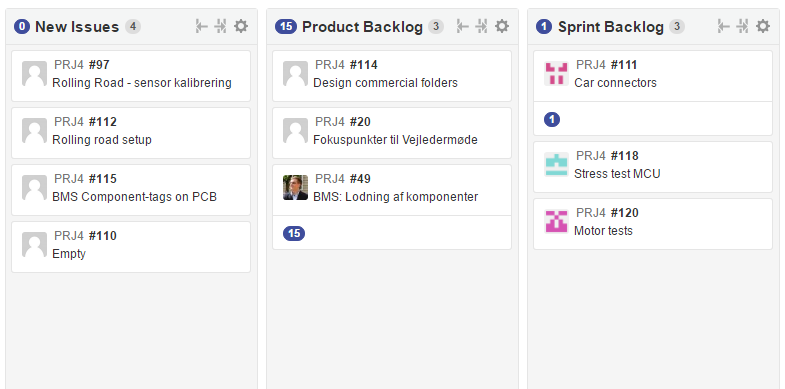
\includegraphics[width=0.7\linewidth]{SubPages/Images/Zenhub1}
	\caption{The 'New issues', 'Product backlog' and 'Sprint backlog' steps}
	\label{fig:Zenhub1}
\end{figure}

\begin{figure}
	\centering
	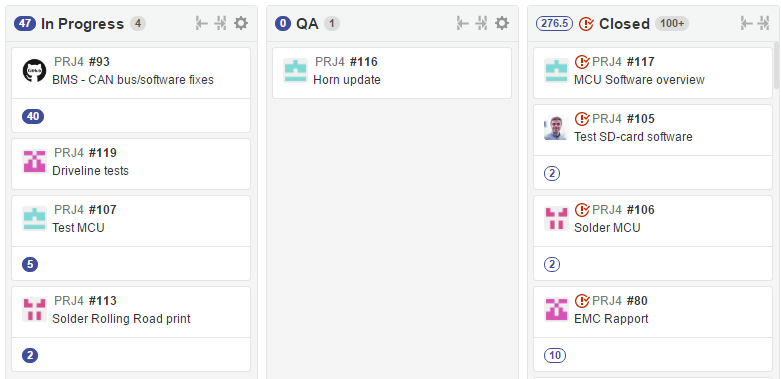
\includegraphics[width=0.7\linewidth]{SubPages/Images/Zenhub2}
	\caption{The 'In progress', 'QA' and 'Closed' steps}
	\label{fig:Zenhub2}
\end{figure}

The sprints was initially divided into two-week periods, but towards the end became one-week periods. The schedule can be seen in the table below:

\begin{tabular}{|c|r|r|}
	\hline \textbf{Sprint} & \textbf{Start date} & \textbf{End date} \\ 
	\hline \#1 & 3/2 & 9/2 \\ 
	\hline \#2 & 9/2 & 23/2 \\ 
	\hline \#3 & 23/2 & 8/3 \\ 
	\hline \#4 & 8/3 & 30/4 \\ 
	\hline Review & & 8/4 \\
	\hline \#5 & 5/4 & 12/4 \\ 
	\hline \#6 & 12/4 & 26/4 \\ 
	\hline \#7 & 26/4 & 10/5 \\ 
	\hline \#8 & 10/5 & 17/7 \\ 
	\hline \#9 & 17/5 & 24/5 \\ 
	\hline Report hand-in &  & 27/5 \\ 
	\hline 
\end{tabular} 

Midway through the project a review was made with an opposing group, where documents was exchanged and reviewed. We sent documents such as requirements and initial design documents.